\section{Why \texorpdfstring{$m_{ij}(t)=1$ does not give $m_{ji}(t)=1$}{m\_ij(t)=1 does not give m\_ji(t)=1}}\label{app:asymmetry}

$m_{ij}(t)$ of Definition~\ref{def:contact} asks whether $i$, at instant $t$, is at a place that
$j$ visits within $\delta$; $m_{ji}(t)$ asks whether $j$, at the same instant, is at a place that
$i$ visits within $\delta$. These are two questions about two different pairs of instants. Both
are read from one set of correspondences $\M_{ij}$, one on each axis, and they agree only if
that set is symmetric about the diagonal $t'=t$. What does hold:
\begin{itemize}
  \item if $m_{ij}(t)=1$ through the pair $(t,t')$, then $m_{ji}(t')=1$: the same pair, read on
        the other axis, $l=t'-t$ later;
  \item every instant of one indicator lies within $\delta$ of an instant of the other;
  \item the contact $a_{ij}=m_{ij}\vee m_{ji}$ is symmetric: $a_{ij}=a_{ji}$.
\end{itemize}
This appendix keeps only the horizontal condition of $\M_{ij}$: the vertical and heading
conditions only remove pairs. $m_{ij}$ fixes the instant of $i$ and lets that of $j$ vary within
$\pm\delta$; $m_{ji}$ fixes the instant of $j$ and lets that of $i$ vary. Nothing makes the two
answers equal.

\subsection{A worked example}

Take $\delta=120$~s and $\varepsilon_h=500$~m, and ignore heights and headings. Pilot $i$ circles
in a thermal at the point $P$ from 0 to 600~s; the radius of the circle is negligible against
$\varepsilon_h$. Pilot $j$ flies east in a straight line at 10~m/s and is in $P$ at 500~s.

\begin{figure}[htbp]
\centering
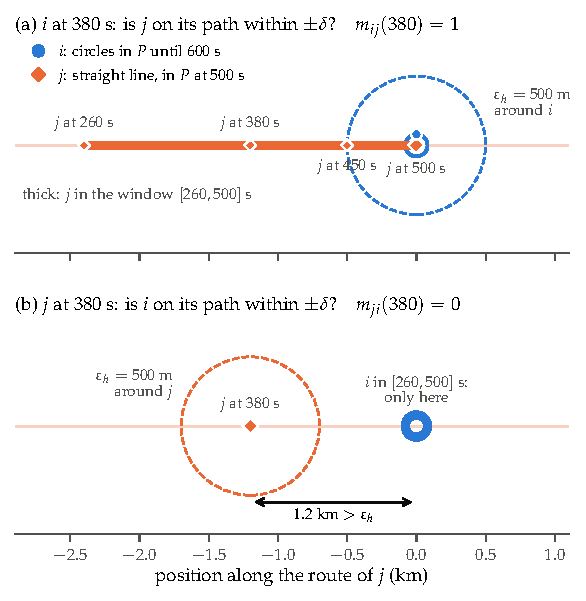
\includegraphics[width=0.74\textwidth]{figures/asymmetry_paths.pdf}
\caption{The example at 380~s. (a)~$i$ is in $P$ and $j$ is 1.2~km west of it. In the window
$[260,500]$~s of $\pm\delta$ (thick), $j$ comes within $\varepsilon_h$ of $i$ at 451~s and is in $P$
at 500~s: the pair $(380,500)$ is a correspondence, so $m_{ij}(380)=1$. (b)~At the same instant
$j$ is 1.2~km from $P$, and during its window $i$ has been only in $P$: no position of $i$ lies
within $\varepsilon_h$ of $j$, so $m_{ji}(380)=0$. The ring only marks $P$.}
\label{fig:asym-paths}
\end{figure}

\begin{table}[htbp]
\centering\small
\begin{tabular}{@{}r l c c c l@{}}
\toprule
$t$ (s) & $j$ relative to $P$ & $m_{ij}$ & $m_{ji}$ & $a_{ij}$ & what happens \\
\midrule
300 & 2.0 km west & 0 & 0 & 0 & $j$ needs more than 120~s to come within 500~m of $P$ \\
380 & 1.2 km west & 1 & 0 & 1 & $i$ is where $j$ will be 120~s later; $j$ is not yet where $i$ has been \\
500 & in $P$ & 1 & 1 & 1 & both are in $P$ \\
560 & 0.6 km east & 1 & 0 & 1 & $i$ is where $j$ was 60~s earlier; $j$ has left \\
\bottomrule
\end{tabular}
\caption{The four instants of the example. Over the whole flight $m_{ij}=1$ from 331 to 600~s,
$m_{ji}=1$ from 451 to 549~s, and $a_{ij}=1$ from 331 to 600~s (strict inequality: exactly
500~m does not count).}
\label{tab:asym-instants}
\end{table}

\subsection{The same example in the plane \texorpdfstring{$(t,t')$}{(t,t')}}

Plot every correspondence $(t,t')$ with the instant at which $i$ passes across and the one at
which $j$ passes up (Figure~\ref{fig:asym-plane}a). Then $m_{ij}(t)=1$ exactly when the
\emph{vertical} line at $t$ meets $\M_{ij}$, and $m_{ji}(t)=1$ exactly when the
\emph{horizontal} line at height $t$ meets it. The two indicators are the shadows of $\M_{ij}$
on the two axes.

At $t=380$ the vertical line meets $\M_{ij}$ (at the pair $(380,500)$ and the ones just below it),
and the horizontal line does not: $\M_{ij}$ has no point with $t'<451$. The set is not symmetric
about the diagonal. The mirror of the pair $(380,500)$ would be $(500,380)$, which needs $i$ at
500~s within 500~m of $j$ at 380~s, and that is 1.2~km away.

\begin{figure}[htbp]
\centering
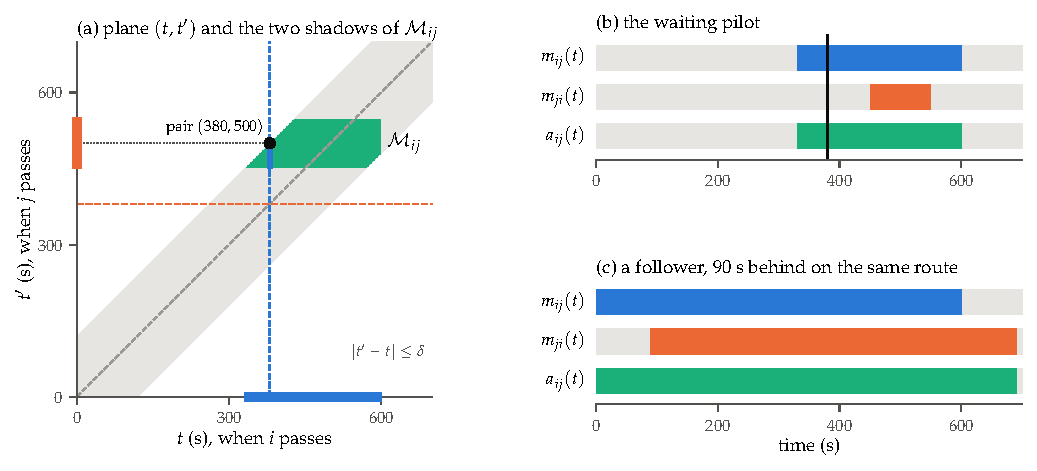
\includegraphics[width=0.94\textwidth]{figures/asymmetry_plane.pdf}
\caption{(a)~The correspondences $\M_{ij}$ (green) in the band $|t'-t|\le\delta$, and its
shadows $m_{ij}$ (blue bar on the $t$ axis) and $m_{ji}$ (orange bar on the $t'$ axis). The
vertical line at 380~s meets $\M_{ij}$ (thick segment), the horizontal one does not. (b)~The
indicators over time, with the line at 380~s. (c)~A pilot $j$ on the same route 90~s behind
$i$: $m_{ji}$ is $m_{ij}$ delayed by exactly 90~s.}
\label{fig:asym-plane}
\end{figure}

\subsection{How far apart they can be}

\textbf{Claim.} If $m_{ij}(t)=1$ there is an instant $t'$ with $|t'-t|\le\delta$ and $m_{ji}(t')=1$;
and conversely.

\emph{Proof.} Take the pair $(t,t')\in\M_{ij}$ that gives $m_{ij}(t)=1$. Then $|t'-t|\le\delta$ by
the definition of $\M_{ij}$, and $m_{ji}(t')=1$ by the definition of $m_{ji}$. The converse is the
same argument read the other way. \hfill$\square$

So the two indicators can differ only by a shift of at most $\delta$. The bound is reached in the
example: the first instant of $m_{ij}$ (331~s) is exactly $\delta$ before the first instant of
$m_{ji}$ (451~s). The union $a_{ij}$ inherits it: at each end of a contact it extends the shorter
indicator by up to $\delta$.

\subsection{Why the contact is the union}

\begin{table}[htbp]
\centering\footnotesize
\begin{tabular}{@{}l c l l@{}}
\toprule
definition & symmetric & in the example & remark \\
\midrule
$m_{ij}\vee m_{ji}$ (used) & yes & 331--600 s & counts the approach and the departure within $\delta$ \\
$m_{ij}\wedge m_{ji}$ & yes & 451--549 s & shorter: each on the path of the other at once \\
$m_{ij}$ alone & no & 331--600 s, or 451--549 s for $(j,i)$ & depends on which pilot is called $i$ \\
\bottomrule
\end{tabular}
\caption{Three ways to define the contact of a pair.}
\label{tab:asym-union}
\end{table}

The union makes the contact independent of the order of the two pilots and keeps the approach and
the departure, where one of them is already on the path of the other. The price is that a contact
starts up to $\delta$ before the pilots are close at the same time. The mutual version
$m_{ij}\wedge m_{ji}$ would give shorter contacts: the false discovery rate and $\tau^*$ would have
to be computed again with the null model, which is not done here.

\textbf{In the code.} \texttt{contacts.scan} returns the instants of $m_{ij}=1$ and, separately,
those of $m_{ji}=1$; \texttt{contacts.pair\_\allowbreak intervals} takes their union. Scenarios:
\texttt{models.WAIT}, \texttt{models.FOLLOW}; figures: \texttt{plots.asymmetry}; numbers checked
in \texttt{test\_note.py}.
